\subchapter
{Basic Buildroot usage}
{Objectives:
  \begin{itemize}
  \item Get Buildroot
  \item Configure a minimal system with Buildroot for the BeagleBone
    Black
  \item Do the build
  \item Prepare the BeagleBone Black for usage
  \item Flash and test the generated system
  \end{itemize}
}

\section{Setup}

Go to the {\tt \$HOME/\longname-labs/} directory.

As specified in the Buildroot
manual\footnote{\url{http://buildroot.org/downloads/manual/manual.html\#requirement-mandatory}},
Buildroot requires a few packages to be installed on your
machine. Let's install them using Ubuntu's package manager:

\begin{verbatim}
sudo apt-get install sed make binutils gcc g++ bash patch \
  gzip bzip2 perl tar cpio python unzip rsync wget libncurses-dev
\end{verbatim}

\section{Download Buildroot}

Since we're going to do Buildroot development, let's clone the
Buildroot source code from its Git repository:

\begin{verbatim}
git clone git://git.busybox.net/buildroot
\end{verbatim}

If your company blocks the {\em Git} protocol (they should not!), then
you can try to clone over HTTP:

\begin{verbatim}
git clone http://git.buildroot.net/git/buildroot.git
\end{verbatim}

In the worst case, if neither work, you can download the Buildroot
tarball \code{buildroot-2016.5.tar.bz2} from
\code{http://buildroot.org/downloads/} and extract it. However in this
case, you won't be able to use {\em Git} to visualize your changes and
keep track of them.

Go into the newly created \code{buildroot} directory.

We're going to start a branch from the {\em 2016.05} Buildroot
release, with which this training has been tested.

\begin{verbatim}
git checkout -b felabs 2016.05
\end{verbatim}

\section{Configuring Buildroot}

If you look under \code{configs/}, you will see that there is a file
named \code{beaglebone_defconfig}, which is a ready-to-use Buildroot
configuration file to build a system for the BeagleBone Black
platform. However, since we want to learn about Buildroot, we'll start
our own configuration from scratch!

Start the Buildroot configuration utility:

\begin{verbatim}
make menuconfig
\end{verbatim}

Of course, you're free to try out the other configuration utilities
\code{nconfig}, \code{xconfig} or \code{gconfig}.

Now, let's do the configuration:

\begin{itemize}

\item \code{Target Options} menu

  \begin{itemize}

  \item It is quite well known that the BeagleBone Black is an ARM based
    platform, so select \code{ARM (little endian)} as the target
    architecture.

  \item According to the BeagleBone Black website at
    \url{http://beagleboard.org/BLACK}, it uses a Texas Instruments
    AM335x, which is based on the ARM Cortex-A8 code. So select
    \code{cortex-A8} as the \code{Target Architecture Variant}.

  \item On ARM two {\em Application Binary Interfaces} are available:
    \code{EABI} and \code{EABIhf}. Unless you have backward
    compatibility concerns with pre-built binaries, \code{EABIhf} is
    more efficient, so make this choice as the \code{Target ABI}
    (which should already be the default anyway).

  \item The other parameters can be left to their default value:
    \code{ELF} is the only available \code{Target Binary Format},
    \code{VFPv3-D16} is a sane default for the {\em Floating Point
      Unit}, and using the \code{ARM} instruction set is also a good
    default (we could use the \code{Thumb-2} instruction set for
    slightly more compact code).

  \end{itemize}

\item We don't have anything special to change in the
  \code{Build options} menu, but take nonetheless this opportunity to
  visit this menu, and look at the available options. Each option has
  a help text that tells you more about the option.

\item \code{Toolchain} menu

  \begin{itemize}

  \item By default, Buildroot builds its own toolchain. This takes
    quite a bit of time, and for \code{ARMv7} platforms, there is a
    pre-built toolchain provided by Linaro. We'll use it through the
    {\em external toolchain} mechanism of Buildroot. Select
    \code{External toolchain} as the \code{Toolchain type}. Do not
    hesitate however to look at the available options when you select
    \code{Buildroot toolchain} as the \code{Toolchain type}.

  \item Select \code{Linaro 2016.02} as the
    \code{Toolchain}. Buildroot can either use pre-defined toolchains
    such as the Linaro one, or custom toolchains (either downloaded
    from a given location, or pre-installed on your machine). Note
    that the Linaro toolchain version might be different if your
    development machine is x86 32 bits and not x86 64 bits.

  \end{itemize}

\item \code{System configuration} menu

  \begin{itemize}

  \item For our basic system, we don't need a lot of custom {\em
      system configuration} for the moment. So take some time to look
    at the available options, and put some custom values for the
    \code{System hostname}, \code{System banner} and \code{Root
      password}.

  \end{itemize}

\item \code{Kernel} menu

  \begin{itemize}

  \item We obviously need a Linux kernel to run on our platform, so
    enable the \code{Linux kernel} option.

  \item By default, the most recent Linux kernel version available at
    the time of the Buildroot release is used. In our case, we want to
    use a specific version: \code{4.6}. So select \code{Custom
      version} as the \code{Kernel version}, and enter \code{4.6} in
    the \code{Kernel version} text field that appears.

  \item Now, we need to define which kernel configuration to
    use. We'll start by using a default configuration provided within
    the kernel sources themselves, called a {\em defconfig}. To
    identify which {\em defconfig} to use, you can look in the kernel
    sources directly, at
    \url{http://git.kernel.org/cgit/linux/kernel/git/torvalds/linux.git/tree/arch/arm/configs/?id=v4.6}. In
    practice, for this platform, it is not trivial to find which one
    to use: the AM335x processor is supported in the Linux kernel as
    part of the support for many other Texas Instruments processors:
    OMAP2, OMAP3, OMAP4, etc. So the appropriate {\em defconfig} is
    named \code{omap2plus_defconfig}. You can open up this file in the
    Linux kernel Git repository viewer, and see it contains the line
    \code{CONFIG_SOC_AM33XX=y}, which is a good indication that it has
    the support for the processor used in the BeagleBone Black. Now
    that we have identified the {\em defconfig} name, enter
    \code{omap2plus} in the \code{Defconfig name} option.

  \item The \code{Kernel binary format} is the next option. Since we
    are going to use a recent U-Boot bootloader, we'll keep the
    default of the \code{zImage} format. The \code{uImage} format used
    to be the norm on ARM platforms, but everybody is now
    transitioning to the \code{zImage} format.

  \item On ARM, most of the platforms now use the {\em Device Tree} to
    describe the hardware. The BeagleBone Black is in this situation,
    so you'll have to enable the \code{Build a Device Tree Blob}
    option. At
    \url{http://git.kernel.org/cgit/linux/kernel/git/torvalds/linux.git/tree/arch/arm/boot/dts/?id=v4.6},
    you can see the list of all Device Tree files available in the 4.6
    Linux kernel (note: the Device Tree files for boards use the
    \code{.dts} extension). The one for the BeagleBone Black is
    \code{am335x-boneblack.dts}. Even if talking about Device Tree is
    beyond the scope of this training, feel free to have a look at
    this file to see what it contains. Back in Buildroot, use the
    option \code{Use a device tree present in the kernel}, and type
    \code{am335x-boneblack} as the \code{Device Tree Source file
      names}.

  \end{itemize}

\item \code{Target packages} menu. This is probably the most important
  menu, as this is the one where you can select amongst the 1800+
  available Buildroot packages which ones should be built and
  installed in your system. For our basic system, enabling
  \code{Busybox} is sufficient and is already enabled by default, but
  feel free to explore the available packages. We'll have the
  opportunity to enable some more packages in the next labs.

\item \code{Filesystem images} menu. For now, keep only the \code{tar
    the root filesystem} option enabled. We'll take care separately of
  flashing the root filesystem on the SD card.

\item \code{Bootloaders} menu.

  \begin{itemize}

  \item We'll use the most popular ARM bootloader, {\em U-Boot}, so
    enable it in the configuration.

  \item Select \code{Kconfig} as the \code{Build system}. U-Boot is
    transitioning from a situation where all the hardware platforms
    were described in C header files to a system where U-Boot re-uses
    the Linux kernel configuration logic. Since we are going to use a
    recent enough U-Boot version, we are going to use the latter,
    called {\em Kconfig}.

  \item You can keep using the default \code{2016.03} version as the
    U-Boot version.

  \item Look at
    \url{http://git.denx.de/?p=u-boot.git;a=tree;f=configs} to
    identify the available U-Boot configuration. The one matching the
    BeagleBone Black is \code{am335x_boneblack_defconfig}, so type
    \code{am335x_boneblack} in \code{Board defconfig}.

  \item U-Boot on AM335x is split in two parts: the first stage
    bootloader called \code{MLO} and the second stage bootloader
    called \code{u-boot.img}. So, select \code{u-boot.img} as the
    \code{U-Boot binary format}, enable \code{Install U-Boot SPL
      binary image} and use \code{MLO} as the \code{U-Boot SPL binary
      image name}.

  \end{itemize}

\end{itemize}

You're now done with the configuration!

\section{Building}

You could simply run \code{make}, but since we would like to keep a
log of the build, we'll redirect both the standard and error outputs
to a file, as well as the terminal by using the \code{tee} command:

\begin{verbatim}
make 2>&1 | tee build.log
\end{verbatim}

While the build is on-going, please go through the following sections
to prepare what will be needed to test the build results.

\section{Prepare the BeagleBone Black}

The BeagleBone Black is powered via the USB-A to mini-USB cable,
connected to the mini-USB connector labeled \code{P4} on the back of
the board.

The Beaglebone serial connector is exported on the 6 male pins close
to one of the 48 pins headers. Using your special USB to Serial
adapter provided by your instructor, connect the ground wire (blue) to
the pin closest to the power supply connector (let's call it pin 1),
and the \code{TX} (red) and \code{RX} (green) wires to the pins 4
(board \code{RX}) and 5 (board \code{TX})\footnote{See
  \url{https://www.olimex.com/Products/Components/Cables/USB-Serial-Cable/USB-Serial-Cable-F/}
  for details about the USB to Serial adapter that we are using.}.

You always should make sure that you connect the \code{TX} pin of the
cable to the \code{RX} pin of the board, and vice-versa, whatever the
board and cables that you use.

\begin{center}
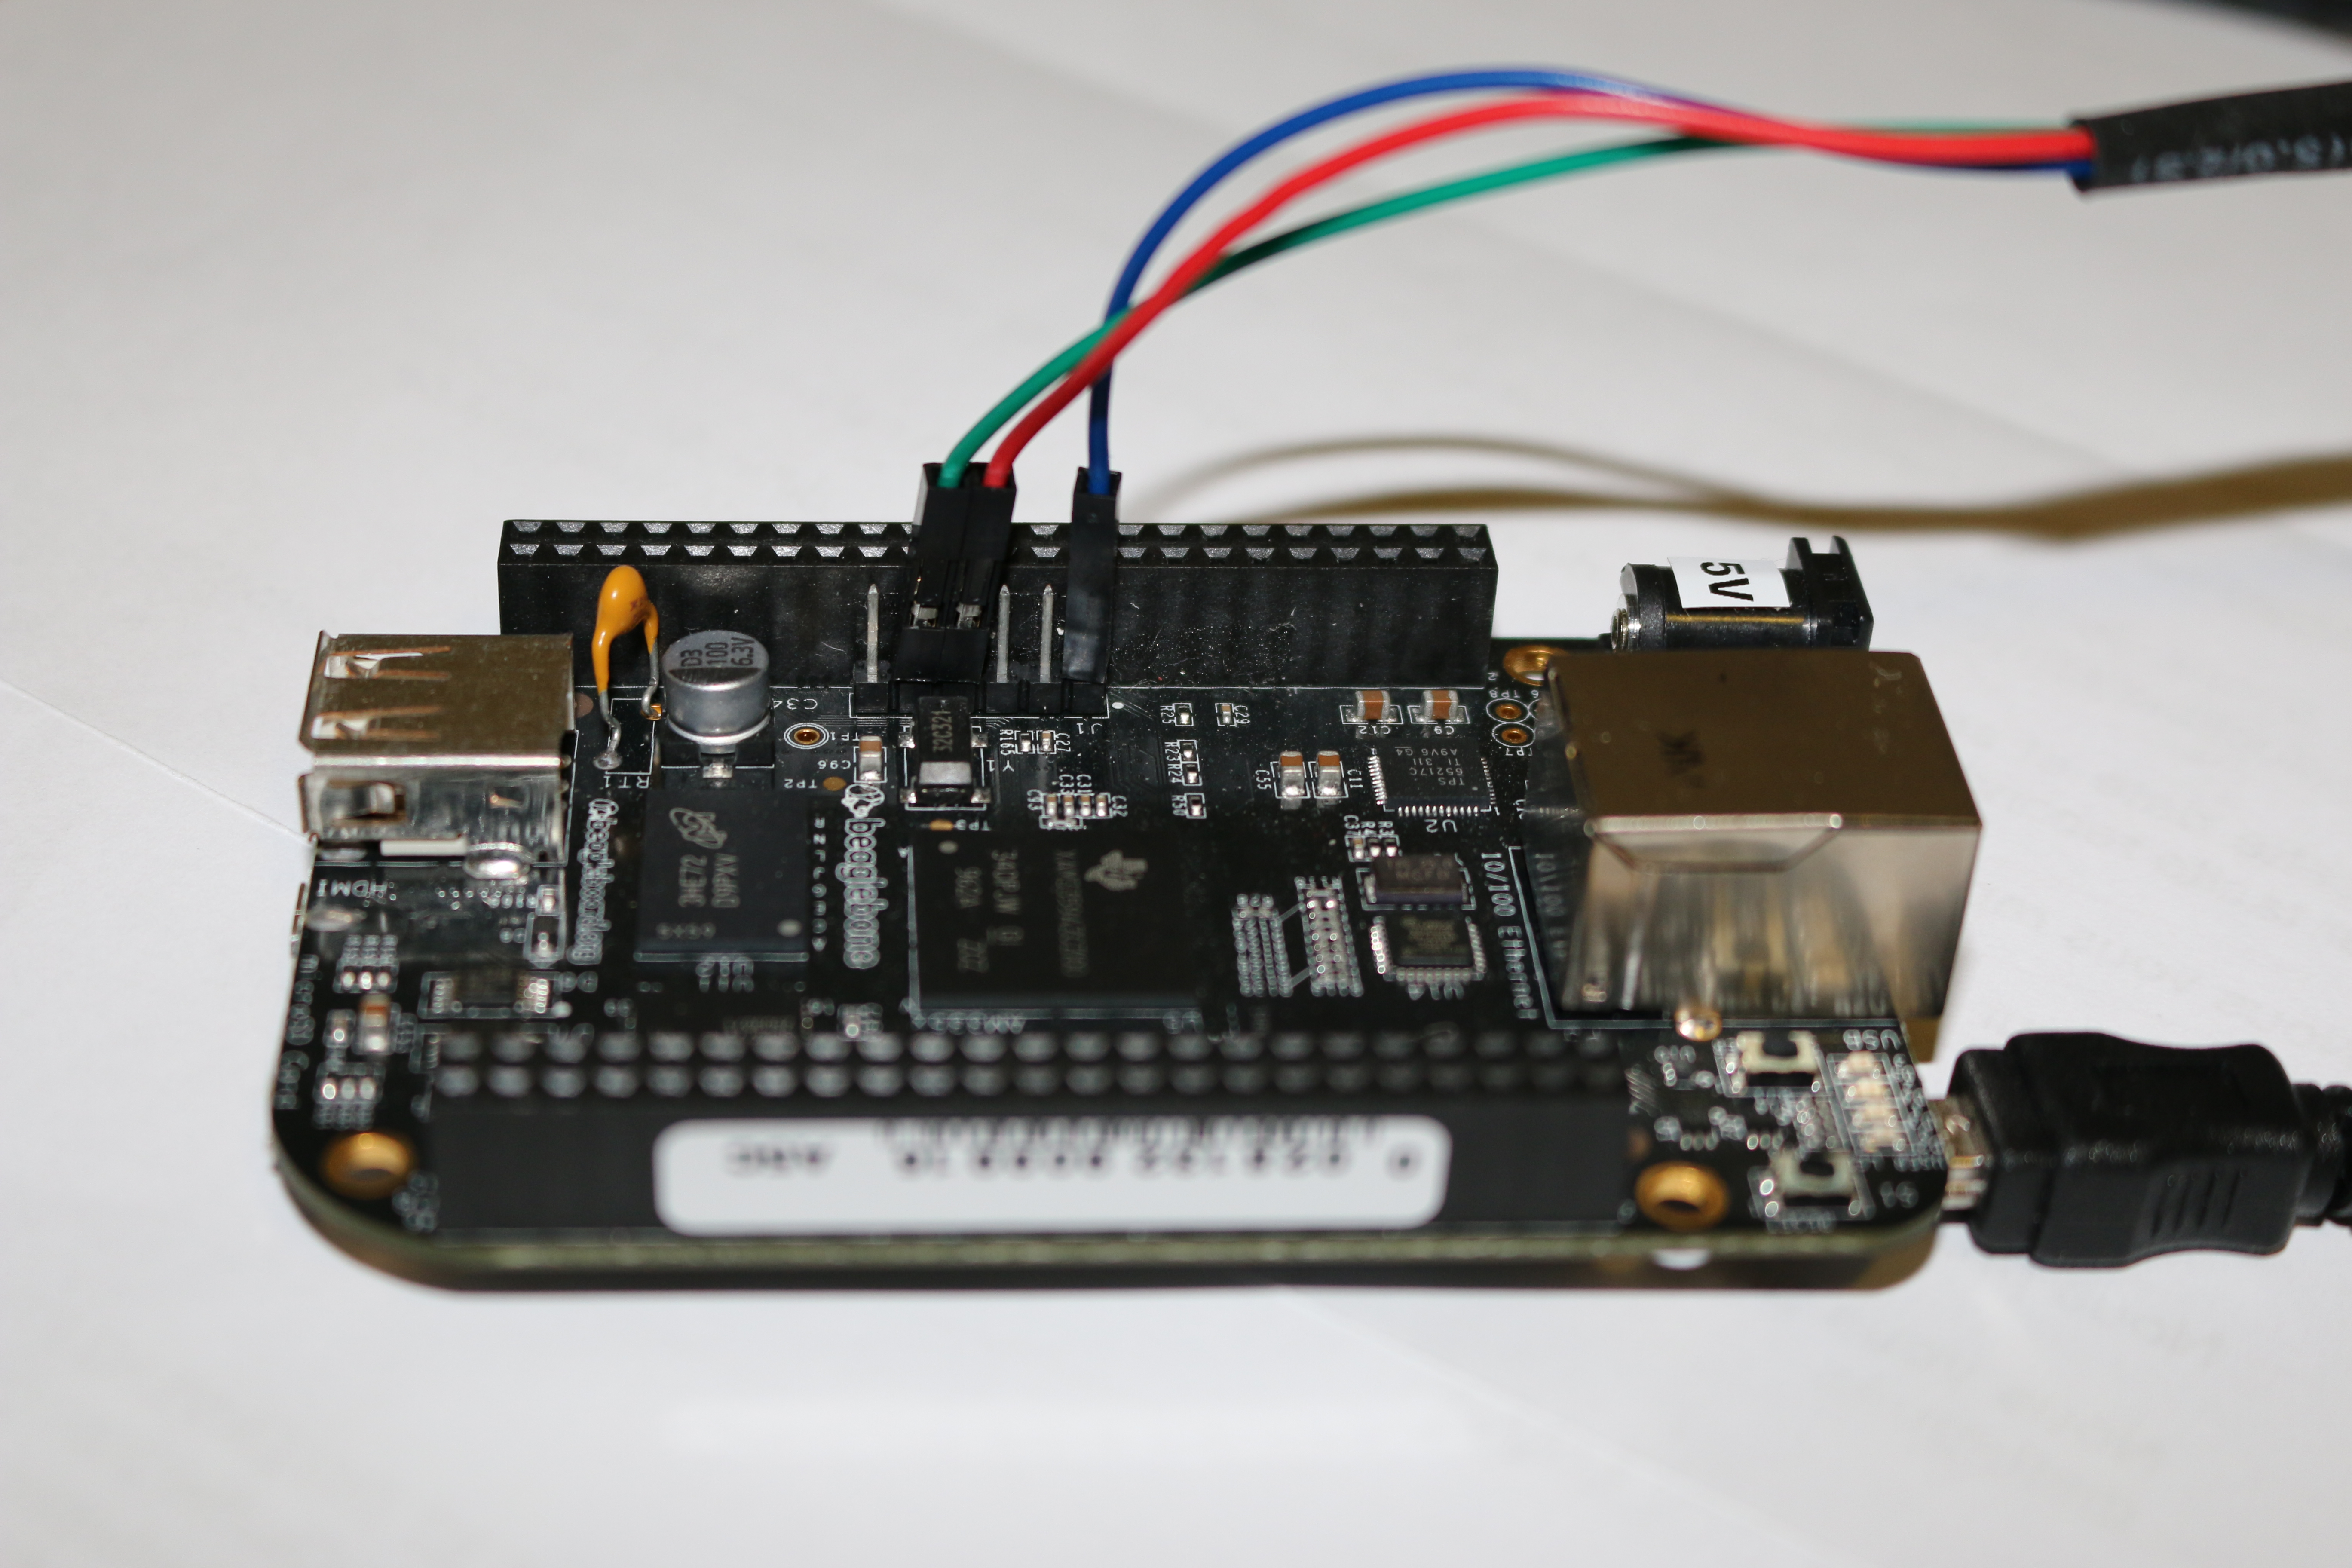
\includegraphics[width=8cm]{labs/buildroot-basic/beaglebone-black-serial-connection.jpg}
\end{center}

Once the USB to Serial connector is plugged in, a new serial port
should appear: \code{/dev/ttyUSB0}.  You can also see this device
appear by looking at the output of \code{dmesg}.

To communicate with the board through the serial port, install a
serial communication program, such as \code{picocom}:

\begin{verbatim}
sudo apt-get install picocom
\end{verbatim}

If you run \code{ls -l /dev/ttyUSB0}, you can also see that only
\code{root} and users belonging to the \code{dialout} group have read
and write access to this file. Therefore, you need to add your user to
the \code{dialout} group:

\begin{verbatim}
sudo adduser $USER dialout
\end{verbatim}

You now need to log out and log in again so that the system actually
sees your user as being part of the {\em dialout} group.

Now, you can run \code{picocom -b 115200 /dev/ttyUSB0}, to start
serial communication on \code{/dev/ttyUSB0}, with a baudrate of
\code{115200}. If you wish to exit \code{picocom}, press
\code{[Ctrl][a]} followed by \code{[Ctrl][x]}.

There should be nothing on the serial line so far, as the board is not
powered up yet.

\section{Prepare the SD card}

Our SD card needs to be split in two partitions:

\begin{itemize}

\item A first partition for the bootloader. It needs to comply with
  the requirements of the AM335x so that it can find the bootloader in
  this partition. It should be a FAT16 partition. We will store the
  bootloader (\code{MLO} and \code{u-boot.img}), the kernel image
  (\code{zImage}), the Device Tree (\code{am335x-boneblack.dtb}) and a
  special U-Boot script for the boot.

\item A second partition for the root filesystem. It can use
  whichever filesystem type you want, but for our system, we'll use
  {\em ext4}.

\end{itemize}

First, let's identify under what name your SD card is identified in
your system: look at the output of \code{cat /proc/partitions} and
find your SD card. In general, if you use the internal SD card reader
of a laptop, it will be \code{mmcblk0}, while if you use an external
USB SD card reader, it will be \code{sdX} (i.e\code{sdb}, \code{sdc},
etc.). {\bf Be careful: \code{/dev/sda} is generally the hard drive of
  your machine!}.

If your SD card is \code{/dev/mmcblk0}, then the partitions inside the
SD card are named \code{mmcblk0p1}, \code{mmc0blkp2}, etc. If your SD
card is \code{/dev/sdc}, then the partitions inside are named
\code{/dev/sdc1}, \code{/dev/sdc2}, etc.

To format our SD card, do the following steps:

\begin{enumerate}

\item Unmount all partitions of your SD card (they are generally
  automatically mounted by Ubuntu)

\item Erase the beginning of the SD card to ensure that the existing
  partitions are not going to be mistakenly detected:\\
  \code{sudo dd if=/dev/zero of=/dev/mmcblk0 bs=1M count=16}. Use
  \code{sdc} or \code{sdb} instead of \code{mmcblk0} if needed.

\item Create the two partitions.

  \begin{itemize}

  \item Start the \code{cfdisk} tool for that:\\
    \code{sudo cfdisk /dev/mmcblk0}.

  \item Chose the {\em dos} partition table type

  \item Create a first small partition (16 MB or 32 MB), primary, with
    type \code{e} ({\em W95 FAT16}) and mark it bootable

  \item Create a second partition, also primary, with the rest of the
    available space, with type \code{83} ({\em Linux}).

  \item Exit \code{cfdisk}

  \end{itemize}

\item Format the first partition as a {\em FAT16} filesystem:\\
  \code{sudo mkfs.vfat -F 16 -n boot /dev/mmcblk0p1}. Use \code{sdc1}
  or \code{sdb1} instead of \code{mmcblk0p1} if needed.

\item Format the second partition as an {\em ext4} filesystem:\\
  \code{sudo mkfs.ext4 -L rootfs -E nodiscard /dev/mmcblk0p2}. Use
  \code{sdc2} or \code{sdb2} instead of \code{mmcblk0p2} if needed.

\end{enumerate}

Remove the SD card and insert it again, the two partitions should be
mounted automatically, in \code{/media/<user>/boot} and
\code{/media/<user>/rootfs}.

Now everything should be ready. Hopefully by that time the Buildroot
build should have completed. If not, wait a little bit more.

\section{Flash the system}

Once Buildroot has finished building the system, it's time to put it
on the SD card:

\begin{itemize}

\item Copy the \code{MLO}, \code{u-boot.img}, \code{zImage} and
  \code{am335x-boneblack.dtb} files from \code{output/images/} to the
  \code{boot} partition of the SD card.

\item Extract the \code{rootfs.tar} file to the \code{rootfs}
  partition of the SD card, using:\\
  \code{sudo tar -C /media/<user>/rootfs/ -xf output/images/rootfs.tar}.

\item Create a file named \code{uEnv.txt} in the \code{boot}
  partition. This file should contain the following lines:

{\small
\begin{verbatim}
bootdir=
bootpart=0:1
uenvcmd=run loadimage;run loadramdisk;run findfdt;run loadfdt;run mmcloados
\end{verbatim}
}

  These lines teach the U-Boot bootloader how to load the Linux kernel
  image and the Device Tree, before booting the kernel.

\end{itemize}

Cleanly unmount the two SD card partitions, and eject the SD card.

\section{Boot the system}

Insert the SD card in the BeagleBone Black. Push the S2 button
(located near the USB host connector) and plug the USB power cable
while holding S2. Pushing S2 forces the BeagleBone Black to boot from
the SD card instead of from the internal eMMC.

You should see your system booting. Make sure that the U-Boot SPL and
U-Boot version and build dates match with the current date. Do the
same check for the Linux kernel.

Login as \code{root} on the BeagleBone Black, and explore the
system. Run \code{ps} to see which processes are running, and look at
what Buildroot has generated in \code{/bin}, \code{/lib}, \code{/usr}
and \code{/etc}.

Note: if your system doesn't boot as expected, make sure to reset the
U-Boot environment by running the following U-Boot commands:

\begin{verbatim}
env default -f -a
saveenv
\end{verbatim}

and reset. This is needed because the U-Boot loaded from the SD card
still loads the U-Boot environment from the eMMC. Ask your instructor
for additional clarifications if needed.

\section{Explore the build log}

Back to your build machine, since we redirected the build output to a
file called \code{build.log}, we can now have a look at it to see what
happened. Since the Buildroot build is quite verbose, Buildroot prints
before each important step a message prefixed by the \code{>>>}
sign. So to get an overall idea of what the build did, you can run:

\begin{verbatim}
grep ">>>" build.log
\end{verbatim}

You see the different packages between downloaded, extracted, patched,
configured, built and installed.

Feel free to explore the \code{output/} directory as well.
